% This is modified samplepaper.tex for anonymized submission
% and meeting specific requirements
%
\documentclass[notitlepage]{llncs}
% \documentclass[notitlepage]{article} % notitlepage
%
\usepackage{graphicx}
\usepackage{hyperref} % Uncomment if you need hyperlinks
\renewcommand\UrlFont{\color{blue}\rmfamily} % Uncomment if using hyperref
\usepackage{amsmath}
\usepackage{geometry}

\geometry{a4paper, left=4cm, right=4cm, bottom=4cm}


\begin{document}
%
\title{Computer Graph Exam 1\thanks{Course delivered by UW-Madison}}
%
% Anonymized for submission
%
\institute{Anonymized for Submission}
%
\maketitle
%
\begin{abstract}
Complete solutions with step-by-step explanations and diagrams for the questions you solved incorrectly during the exam to earn 0.25 points (out of 30) for each question (if your answers are typed in Latex or HTML and diagrams are drawn using either Latex or HTML Canvas, you will earn an additional 0.25 points for each question).

\keywords{Computer Graph \and Exam \and Solution}
\end{abstract}

% Use \newpage to ensure each section starts on a new page
\newpage
\section*{Question 8: Rotation and Scaling Matrices}
\textbf{Question:} Which of the following matrices are 2D rotation and scaling matrices at the same time?
\\

\textbf{Choices:}
\begin{enumerate}
\renewcommand{\labelenumi}{\Alph{enumi}.} 
    \item $\begin{bmatrix}
            1 & \ 0 \\
            0 & \ 1
            \end{bmatrix}$\\
    \item $\begin{bmatrix}
            0 & -1 \\
            1 & 0
            \end{bmatrix}$\\
    \item $\begin{bmatrix}
            0 & 1 \\
            -1 & 0
            \end{bmatrix}$\\
    \item $\begin{bmatrix}
            -1 & 0 \\
            0 & -1
            \end{bmatrix}$\\
    \item $\begin{bmatrix}
            0 & 0 \\
            0 & 0
            \end{bmatrix}$\\
    \item None of the other choices
\end{enumerate}

\textbf{Correct Answer:} $\begin{bmatrix}
                            -1 & 0 \\
                            0 & -1
                            \end{bmatrix}$
\\

\textbf{Explanation:}

A 2D rotation matrix for an angle $\theta$ is defined as:
\[ R(\theta) = \begin{bmatrix} \cos\theta & -\sin\theta \\ \sin\theta & \cos\theta \end{bmatrix} \]

A 2D scaling matrix with factors $s_x$ and $s_y$ is defined as:
\[ S(s_x, s_y) = \begin{bmatrix} s_x & 0 \\ 0 & s_y \end{bmatrix} \]

The matrix \([-1, 0], [0, -1]\) can be interpreted as both a scaling matrix (scaling by -1 on both axes, effectively mirroring the image) and a rotation matrix (rotating by 180 degrees, since $\cos180^\circ = -1$ and $\sin180^\circ = 0$).

Thus, \([-1, 0], [0, -1]\) satisfies the criteria for both a 2D rotation matrix and a scaling matrix.

\newpage
\section*{Question 15: Cardinal Spline Derivative}
\textbf{Question:} Which of the following can be the derivative (tangent vector) at \([0, 0]\) for a Cardinal spline (not necessarily Catmull-Rom) interpolating points \([300, 300]\), \([0, 0]\), \([0, 300]\), \([300, 0]\) (in this order)?
\\

\textbf{Choices:}
\begin{enumerate}
\renewcommand{\labelenumi}{\Alph{enumi}.} 
    \item \([-150,0]\)
    \item \([100,0]\)
    \item \([150,0]\)
    \item \([-100,0]\)
    \item \([-200,0]\)
    \item None of the other choices
\end{enumerate}

\textbf{Correct Answer:} \([-100,0]\)
\\

\textbf{Explanation:}

For a Cardinal spline, the derivative at a point \( P_i \) can be given by the tension parameter \( c \) times the difference between the following and preceding points. Considering \( P_1 = [0, 0] \), the derivative \( T_1 \) is calculated as:
\[ T_1 = c \cdot (P_{2} - P_{0}) \]
Given \( P_0 = [300, 300] \) and \( P_2 = [0, 300] \), we find:
\[ T_1 = c \cdot \begin{bmatrix}
                            0 - 300 \\
                            300 - 300
                        \end{bmatrix} \]
\[ T_1 = c \cdot \begin{bmatrix}
                            -300 \\
                            0
                        \end{bmatrix} \]
The correct tangent vector at \([0, 0]\) must be a scalar multiple of this difference. Among the given options, \(\begin{bmatrix}
-100 \\
0
\end{bmatrix}\) is the vector that is a scalar multiple of \(\begin{bmatrix}
-300 \\
0
\end{bmatrix}\), implying that the tension parameter \( c \) is \( \frac{1}{3} \).

\begin{figure}[h]
    \centering
    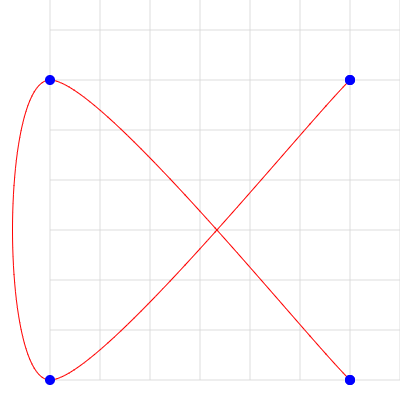
\includegraphics[width=0.45\textwidth]{CardinalSpline.png}
    \caption{Cardinal Spline visualization.}
\end{figure}


\newpage
\section*{Question 26: Cubic and Quadratic Bezier Curves}
\textbf{Question:} Which of the following cubic Bezier curves (given by the ordered list of control points) is the same as the quadratic Bezier curve with control points \([0, 0]\), \([0, 300]\), \([300, 300]\) (in this order)?
\\

\textbf{Choices:}
\begin{enumerate}
\renewcommand{\labelenumi}{\Alph{enumi}.} 
    \item None of the other choices
    \item \([0, 0]\), \([0, 300]\), \([0, 300]\), \([300, 300]\) 
    \item \([0, 0]\), \([0, 450]\), \([-150, 300]\), \([300, 300]\) 
    \item \([0, 0]\), \([0, 100]\), \([200, 300]\), \([300, 300]\) 
    \item It cannot be the same as any cubic curve 
    \item \([0, 0]\), \([0, 200]\), \([100, 300]\), \([300, 300]\)
\end{enumerate}

\textbf{Correct Answer:} \([0, 0]\), \([0, 200]\), \([100, 300]\), \([300, 300]\)
\\

\textbf{Explanation:}

To transform a quadratic Bezier curve with control points \(P_0\), \(P_1\), and \(P_2\) to a cubic one, we derive new control points \(Q_0\), \(Q_1\), \(Q_2\), and \(Q_3\) such that the shapes of the two curves are identical. The cubic control points can be calculated using the relations:

\[ Q_1 = \frac{2}{3}P_1 + \frac{1}{3}P_0 \]
\[ Q_2 = \frac{2}{3}P_1 + \frac{1}{3}P_2 \]

Given the quadratic control points \(P_0 = [0, 0]\), \(P_1 = [0, 300]\), and \(P_2 = [300, 300]\), we compute:

\[ Q_1 = \frac{2}{3}[0, 300] + \frac{1}{3}[0, 0] = [0, 200] \]
\[ Q_2 = \frac{2}{3}[0, 300] + \frac{1}{3}[300, 300] = [100, 300] \]

Thus, the cubic Bezier curve with control points \([0, 0]\), \([0, 200]\), \([100, 300]\), \([300, 300]\) is equivalent to the given quadratic Bezier curve.

\begin{figure}[htbp]
  \centering
  \begin{minipage}[b]{0.4\textwidth}
    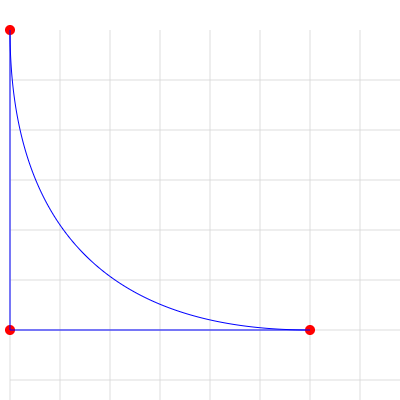
\includegraphics[width=\textwidth]{QuadraticBezierCurve.png}
    \caption{Quadratic Bezier Curve}
  \end{minipage}
  \hfill
  \begin{minipage}[b]{0.4\textwidth}
    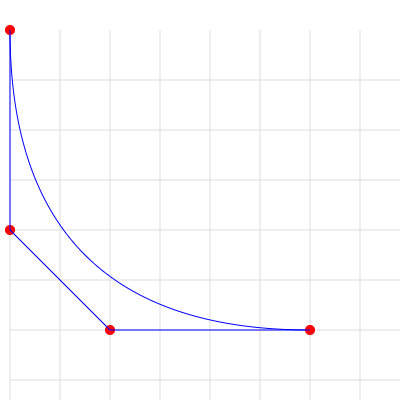
\includegraphics[width=\textwidth]{CubicBezierCurve.png}
    \caption{Cubic Bezier Curve}
  \end{minipage}
\end{figure}



\newpage
\section*{Acknowledgements}
I want to extend my gratitude to the customized GPT model `Taco` for providing assistance and valuable insights that significantly contributed to completing this work.


% References or Bibliography can be added here if necessary

\end{document}
